% Options for packages loaded elsewhere
\PassOptionsToPackage{unicode}{hyperref}
\PassOptionsToPackage{hyphens}{url}
\PassOptionsToPackage{dvipsnames,svgnames,x11names}{xcolor}
%
\documentclass[
  letterpaper,
  DIV=11,
  numbers=noendperiod]{scrreprt}

\usepackage{amsmath,amssymb}
\usepackage{lmodern}
\usepackage{iftex}
\ifPDFTeX
  \usepackage[T1]{fontenc}
  \usepackage[utf8]{inputenc}
  \usepackage{textcomp} % provide euro and other symbols
\else % if luatex or xetex
  \usepackage{unicode-math}
  \defaultfontfeatures{Scale=MatchLowercase}
  \defaultfontfeatures[\rmfamily]{Ligatures=TeX,Scale=1}
\fi
% Use upquote if available, for straight quotes in verbatim environments
\IfFileExists{upquote.sty}{\usepackage{upquote}}{}
\IfFileExists{microtype.sty}{% use microtype if available
  \usepackage[]{microtype}
  \UseMicrotypeSet[protrusion]{basicmath} % disable protrusion for tt fonts
}{}
\makeatletter
\@ifundefined{KOMAClassName}{% if non-KOMA class
  \IfFileExists{parskip.sty}{%
    \usepackage{parskip}
  }{% else
    \setlength{\parindent}{0pt}
    \setlength{\parskip}{6pt plus 2pt minus 1pt}}
}{% if KOMA class
  \KOMAoptions{parskip=half}}
\makeatother
\usepackage{xcolor}
\setlength{\emergencystretch}{3em} % prevent overfull lines
\setcounter{secnumdepth}{5}
% Make \paragraph and \subparagraph free-standing
\ifx\paragraph\undefined\else
  \let\oldparagraph\paragraph
  \renewcommand{\paragraph}[1]{\oldparagraph{#1}\mbox{}}
\fi
\ifx\subparagraph\undefined\else
  \let\oldsubparagraph\subparagraph
  \renewcommand{\subparagraph}[1]{\oldsubparagraph{#1}\mbox{}}
\fi

\usepackage{color}
\usepackage{fancyvrb}
\newcommand{\VerbBar}{|}
\newcommand{\VERB}{\Verb[commandchars=\\\{\}]}
\DefineVerbatimEnvironment{Highlighting}{Verbatim}{commandchars=\\\{\}}
% Add ',fontsize=\small' for more characters per line
\usepackage{framed}
\definecolor{shadecolor}{RGB}{241,243,245}
\newenvironment{Shaded}{\begin{snugshade}}{\end{snugshade}}
\newcommand{\AlertTok}[1]{\textcolor[rgb]{0.68,0.00,0.00}{#1}}
\newcommand{\AnnotationTok}[1]{\textcolor[rgb]{0.37,0.37,0.37}{#1}}
\newcommand{\AttributeTok}[1]{\textcolor[rgb]{0.40,0.45,0.13}{#1}}
\newcommand{\BaseNTok}[1]{\textcolor[rgb]{0.68,0.00,0.00}{#1}}
\newcommand{\BuiltInTok}[1]{\textcolor[rgb]{0.00,0.23,0.31}{#1}}
\newcommand{\CharTok}[1]{\textcolor[rgb]{0.13,0.47,0.30}{#1}}
\newcommand{\CommentTok}[1]{\textcolor[rgb]{0.37,0.37,0.37}{#1}}
\newcommand{\CommentVarTok}[1]{\textcolor[rgb]{0.37,0.37,0.37}{\textit{#1}}}
\newcommand{\ConstantTok}[1]{\textcolor[rgb]{0.56,0.35,0.01}{#1}}
\newcommand{\ControlFlowTok}[1]{\textcolor[rgb]{0.00,0.23,0.31}{#1}}
\newcommand{\DataTypeTok}[1]{\textcolor[rgb]{0.68,0.00,0.00}{#1}}
\newcommand{\DecValTok}[1]{\textcolor[rgb]{0.68,0.00,0.00}{#1}}
\newcommand{\DocumentationTok}[1]{\textcolor[rgb]{0.37,0.37,0.37}{\textit{#1}}}
\newcommand{\ErrorTok}[1]{\textcolor[rgb]{0.68,0.00,0.00}{#1}}
\newcommand{\ExtensionTok}[1]{\textcolor[rgb]{0.00,0.23,0.31}{#1}}
\newcommand{\FloatTok}[1]{\textcolor[rgb]{0.68,0.00,0.00}{#1}}
\newcommand{\FunctionTok}[1]{\textcolor[rgb]{0.28,0.35,0.67}{#1}}
\newcommand{\ImportTok}[1]{\textcolor[rgb]{0.00,0.46,0.62}{#1}}
\newcommand{\InformationTok}[1]{\textcolor[rgb]{0.37,0.37,0.37}{#1}}
\newcommand{\KeywordTok}[1]{\textcolor[rgb]{0.00,0.23,0.31}{#1}}
\newcommand{\NormalTok}[1]{\textcolor[rgb]{0.00,0.23,0.31}{#1}}
\newcommand{\OperatorTok}[1]{\textcolor[rgb]{0.37,0.37,0.37}{#1}}
\newcommand{\OtherTok}[1]{\textcolor[rgb]{0.00,0.23,0.31}{#1}}
\newcommand{\PreprocessorTok}[1]{\textcolor[rgb]{0.68,0.00,0.00}{#1}}
\newcommand{\RegionMarkerTok}[1]{\textcolor[rgb]{0.00,0.23,0.31}{#1}}
\newcommand{\SpecialCharTok}[1]{\textcolor[rgb]{0.37,0.37,0.37}{#1}}
\newcommand{\SpecialStringTok}[1]{\textcolor[rgb]{0.13,0.47,0.30}{#1}}
\newcommand{\StringTok}[1]{\textcolor[rgb]{0.13,0.47,0.30}{#1}}
\newcommand{\VariableTok}[1]{\textcolor[rgb]{0.07,0.07,0.07}{#1}}
\newcommand{\VerbatimStringTok}[1]{\textcolor[rgb]{0.13,0.47,0.30}{#1}}
\newcommand{\WarningTok}[1]{\textcolor[rgb]{0.37,0.37,0.37}{\textit{#1}}}

\providecommand{\tightlist}{%
  \setlength{\itemsep}{0pt}\setlength{\parskip}{0pt}}\usepackage{longtable,booktabs,array}
\usepackage{calc} % for calculating minipage widths
% Correct order of tables after \paragraph or \subparagraph
\usepackage{etoolbox}
\makeatletter
\patchcmd\longtable{\par}{\if@noskipsec\mbox{}\fi\par}{}{}
\makeatother
% Allow footnotes in longtable head/foot
\IfFileExists{footnotehyper.sty}{\usepackage{footnotehyper}}{\usepackage{footnote}}
\makesavenoteenv{longtable}
\usepackage{graphicx}
\makeatletter
\def\maxwidth{\ifdim\Gin@nat@width>\linewidth\linewidth\else\Gin@nat@width\fi}
\def\maxheight{\ifdim\Gin@nat@height>\textheight\textheight\else\Gin@nat@height\fi}
\makeatother
% Scale images if necessary, so that they will not overflow the page
% margins by default, and it is still possible to overwrite the defaults
% using explicit options in \includegraphics[width, height, ...]{}
\setkeys{Gin}{width=\maxwidth,height=\maxheight,keepaspectratio}
% Set default figure placement to htbp
\makeatletter
\def\fps@figure{htbp}
\makeatother
\newlength{\cslhangindent}
\setlength{\cslhangindent}{1.5em}
\newlength{\csllabelwidth}
\setlength{\csllabelwidth}{3em}
\newlength{\cslentryspacingunit} % times entry-spacing
\setlength{\cslentryspacingunit}{\parskip}
\newenvironment{CSLReferences}[2] % #1 hanging-ident, #2 entry spacing
 {% don't indent paragraphs
  \setlength{\parindent}{0pt}
  % turn on hanging indent if param 1 is 1
  \ifodd #1
  \let\oldpar\par
  \def\par{\hangindent=\cslhangindent\oldpar}
  \fi
  % set entry spacing
  \setlength{\parskip}{#2\cslentryspacingunit}
 }%
 {}
\usepackage{calc}
\newcommand{\CSLBlock}[1]{#1\hfill\break}
\newcommand{\CSLLeftMargin}[1]{\parbox[t]{\csllabelwidth}{#1}}
\newcommand{\CSLRightInline}[1]{\parbox[t]{\linewidth - \csllabelwidth}{#1}\break}
\newcommand{\CSLIndent}[1]{\hspace{\cslhangindent}#1}

\KOMAoption{captions}{tableheading}
\makeatletter
\makeatother
\makeatletter
\@ifpackageloaded{bookmark}{}{\usepackage{bookmark}}
\makeatother
\makeatletter
\@ifpackageloaded{caption}{}{\usepackage{caption}}
\AtBeginDocument{%
\ifdefined\contentsname
  \renewcommand*\contentsname{Table of contents}
\else
  \newcommand\contentsname{Table of contents}
\fi
\ifdefined\listfigurename
  \renewcommand*\listfigurename{List of Figures}
\else
  \newcommand\listfigurename{List of Figures}
\fi
\ifdefined\listtablename
  \renewcommand*\listtablename{List of Tables}
\else
  \newcommand\listtablename{List of Tables}
\fi
\ifdefined\figurename
  \renewcommand*\figurename{Figure}
\else
  \newcommand\figurename{Figure}
\fi
\ifdefined\tablename
  \renewcommand*\tablename{Table}
\else
  \newcommand\tablename{Table}
\fi
}
\@ifpackageloaded{float}{}{\usepackage{float}}
\floatstyle{ruled}
\@ifundefined{c@chapter}{\newfloat{codelisting}{h}{lop}}{\newfloat{codelisting}{h}{lop}[chapter]}
\floatname{codelisting}{Listing}
\newcommand*\listoflistings{\listof{codelisting}{List of Listings}}
\makeatother
\makeatletter
\@ifpackageloaded{caption}{}{\usepackage{caption}}
\@ifpackageloaded{subcaption}{}{\usepackage{subcaption}}
\makeatother
\makeatletter
\@ifpackageloaded{tcolorbox}{}{\usepackage[many]{tcolorbox}}
\makeatother
\makeatletter
\@ifundefined{shadecolor}{\definecolor{shadecolor}{rgb}{.97, .97, .97}}
\makeatother
\makeatletter
\makeatother
\ifLuaTeX
  \usepackage{selnolig}  % disable illegal ligatures
\fi
\IfFileExists{bookmark.sty}{\usepackage{bookmark}}{\usepackage{hyperref}}
\IfFileExists{xurl.sty}{\usepackage{xurl}}{} % add URL line breaks if available
\urlstyle{same} % disable monospaced font for URLs
\hypersetup{
  pdftitle={Transcriptome Data Analysis in Non-model Organisms},
  pdfauthor={Ponsit Sathapondecha; Jiratchaya Nuanpirom; Prasert Yodsawat},
  colorlinks=true,
  linkcolor={blue},
  filecolor={Maroon},
  citecolor={Blue},
  urlcolor={Blue},
  pdfcreator={LaTeX via pandoc}}

\title{Transcriptome Data Analysis in Non-model Organisms}
\author{Ponsit Sathapondecha \and Jiratchaya Nuanpirom \and Prasert
Yodsawat}
\date{2/28/23}

\begin{document}
\maketitle
\ifdefined\Shaded\renewenvironment{Shaded}{\begin{tcolorbox}[borderline west={3pt}{0pt}{shadecolor}, boxrule=0pt, interior hidden, enhanced, frame hidden, breakable, sharp corners]}{\end{tcolorbox}}\fi

\renewcommand*\contentsname{Table of contents}
{
\hypersetup{linkcolor=}
\setcounter{tocdepth}{2}
\tableofcontents
}
\bookmarksetup{startatroot}

\hypertarget{preface}{%
\chapter*{Preface}\label{preface}}
\addcontentsline{toc}{chapter}{Preface}

\markboth{Preface}{Preface}

This is a Quarto book.

To learn more about Quarto books visit
\url{https://quarto.org/docs/books}.

\begin{Shaded}
\begin{Highlighting}[]
\DecValTok{1} \SpecialCharTok{+} \DecValTok{1}
\end{Highlighting}
\end{Shaded}

\begin{verbatim}
[1] 2
\end{verbatim}

\bookmarksetup{startatroot}

\hypertarget{introduction-to-mobaxterm-terminal-and-ssh}{%
\chapter{Introduction to MobaXterm, Terminal, and
SSH}\label{introduction-to-mobaxterm-terminal-and-ssh}}

\hypertarget{mobaxterm-for-windows}{%
\section{MobaXterm (for Windows)}\label{mobaxterm-for-windows}}

MobaXterm is a toolbox for remote computing. In a single Windows
application, it provides loads of functions that are tailored for
programmers, webmasters, IT administrators and pretty much all users who
need to handle their remote jobs in a more simple fashion. MobaXterm
provides all the important remote network tools, such as SSH, X11, RDP,
VNC, FTP, MOSH, and of course, Unix commands, and many more!

\begin{figure}

{\centering 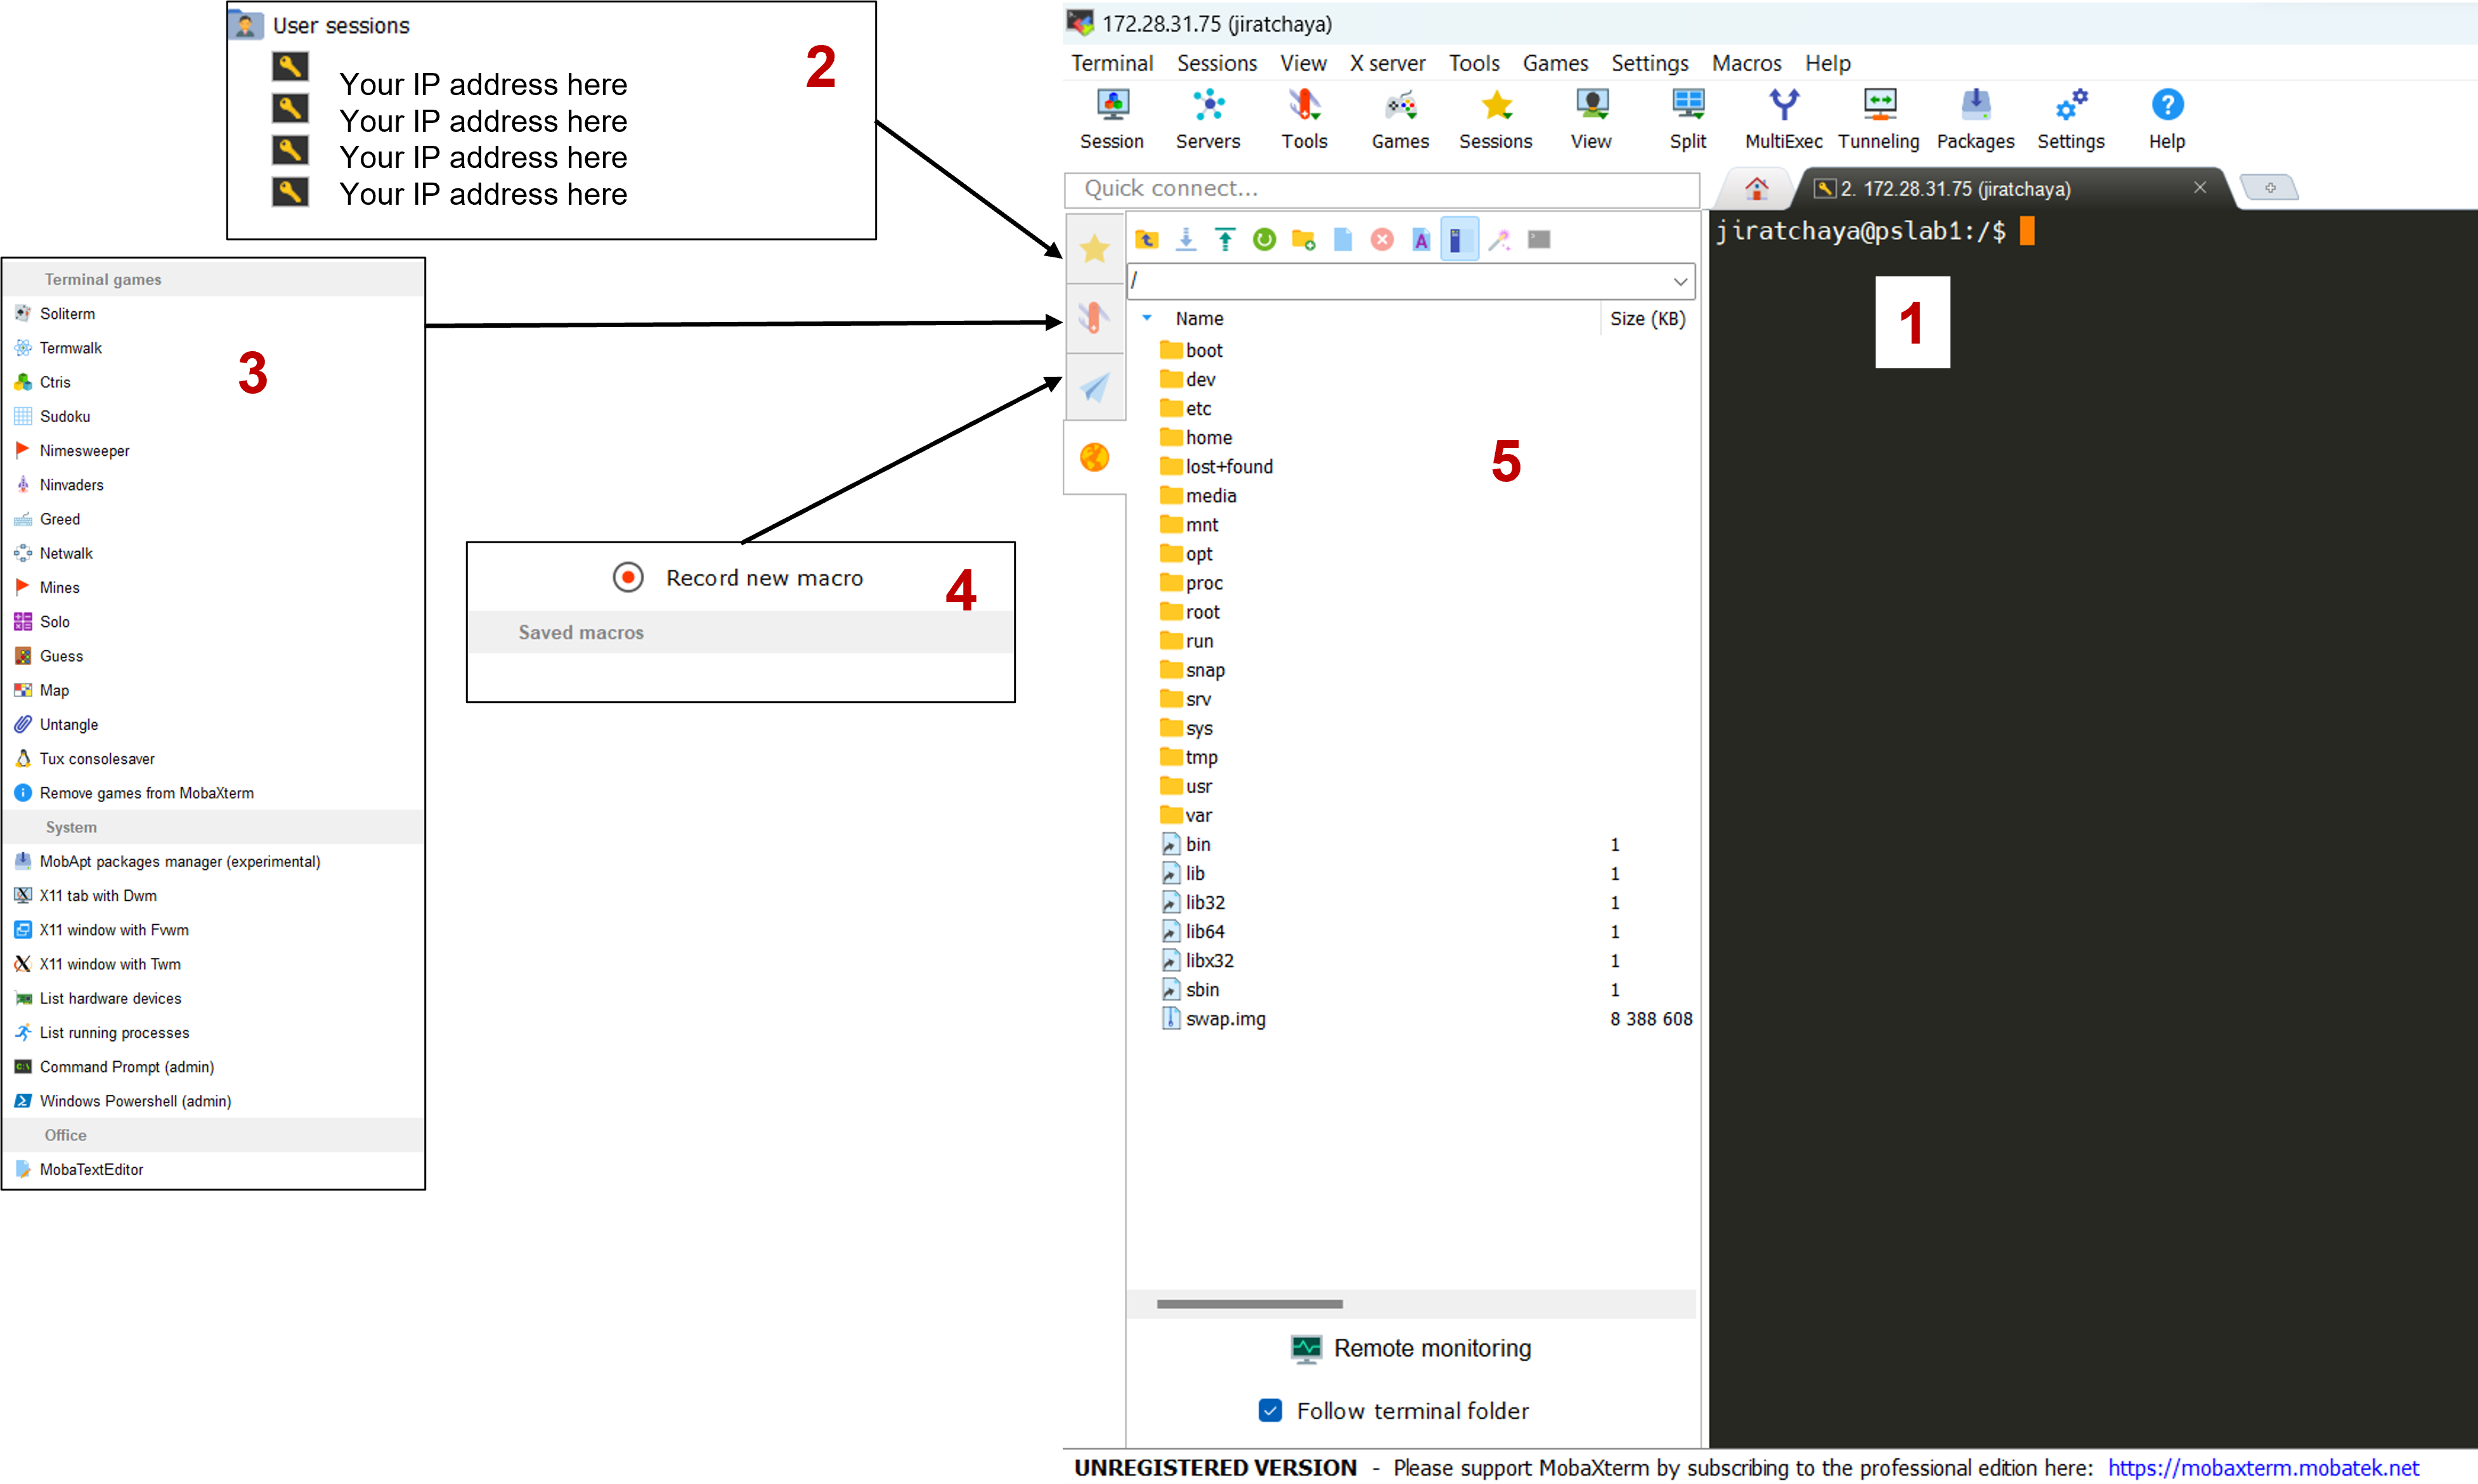
\includegraphics{./assets/01_moba_ui.png}

}

\caption{MobaXterm user interface. In the context of remote access
through SSH and FTP, mobaXterm provides easy-to-access route as (1) a
secure shell (SSH) terminal of the remote server, (2) a list of remote
server you've accessed, (3) Utilities facilitating remote server access
including entertainment, like Swiss army knife!, (4) If you want to
reduce redundant typing, just set macro to it, and (5) a files available
in the current working directory in the remote server, you can also
transfer files from remote server to your local computer using this
route!}

\end{figure}

There are many advantages of having an All-In-One network application
for your remote tasks, e.g.~when you use SSH to connect to a remote
server, a graphical SFTP browser will automatically pop up in order to
directly edit your remote files.

Visit MobaXterm official website to see a demo:
https://mobaxterm.mobatek.net/demo.html

\hypertarget{terminal-for-macos}{%
\section{Terminal (for macOS)}\label{terminal-for-macos}}

Terminal provides a command-line interface to macOS. Each window in
Terminal represents an instance of a shell process. The window contains
a prompt that indicates you can enter a command. The prompt you see
depends on your Terminal and shell settings, but it often includes the
name of the host you're logged in to, your current working folder, your
user name, and a prompt symbol. For example, if a user named michael is
using the default zsh shell, the prompt appears as:

\begin{verbatim}
michael@MacBook-Pro ~ %
\end{verbatim}

This indicates that the user named michael is logged in to a computer
named MacBook-Pro, and the current folder is his home folder, indicated
by the tilde (\textasciitilde).

MacOS features a built-in SSH client called Terminal which allows you to
quickly and easily connect to a server. Starting from open the
``terminal'' app, and enter the standard SSH command:

\begin{verbatim}
ssh user@IPAddress
\end{verbatim}

This will connect to the server via SSH with the username `user` and the
default SSH port 22. The connection will look similar to the following:

\hypertarget{connecting-to-remote-server}{%
\section{Connecting to Remote
Server}\label{connecting-to-remote-server}}

Bioinformatics data processing tasks require more computing power than
our laptops, so we need large servers or clusters. It's likely you'll
work mostly over a network connection with remote machines on some
projects. It can be frustrating for beginners to work with a remote
machine. So, This part will introduce you to some commonly used bash
commands. To make it easier for beginners to manage their remote
machines, there are a range of different tools and technologies
available, such as SSH, FTP, and terminal commands, which can be used to
access and manage the environment of the machine. Additionally, there
are a variety of bash commands which can be used to streamline the
process of managing the machine.

What you need to know for connecting to a remove server:

\begin{enumerate}
\def\labelenumi{\arabic{enumi}.}
\item
  Your username and password in the remote server
\item
  IP address of the remote server, and which port to connect to server
\item
  You should know whether the remote server accessible via local network
  or a public IP address
\end{enumerate}

By default, SSH uses port 22 but it can be changed to a non-standard
port. To securely connect the client to the remote server, SSH uses
symmetric encryption, asymmetric encryption, and hashing. If you're
connecting for the first time, you'll be asked to verify the server's
public key. Whenever you connect to the same server in the future, the
client will reference this verified public key. During an SSH
connection, the client and server negotiate a session key used to
encrypt and decrypt data.

\begin{figure}

{\centering 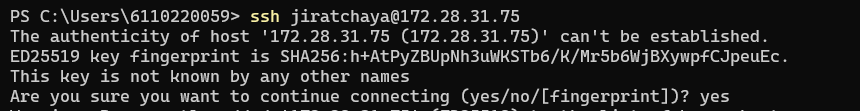
\includegraphics{./assets/02_ssh_authkeys.png}

}

\caption{In order to establish a connection, SSH needs to verify SHA
keys once connected for the first time. Once authentication is complete,
the SSH connection is secure and can be trusted for future access.}

\end{figure}

Upon connecting to the remote server, you'll see a welcome message like
this

\begin{figure}

{\centering 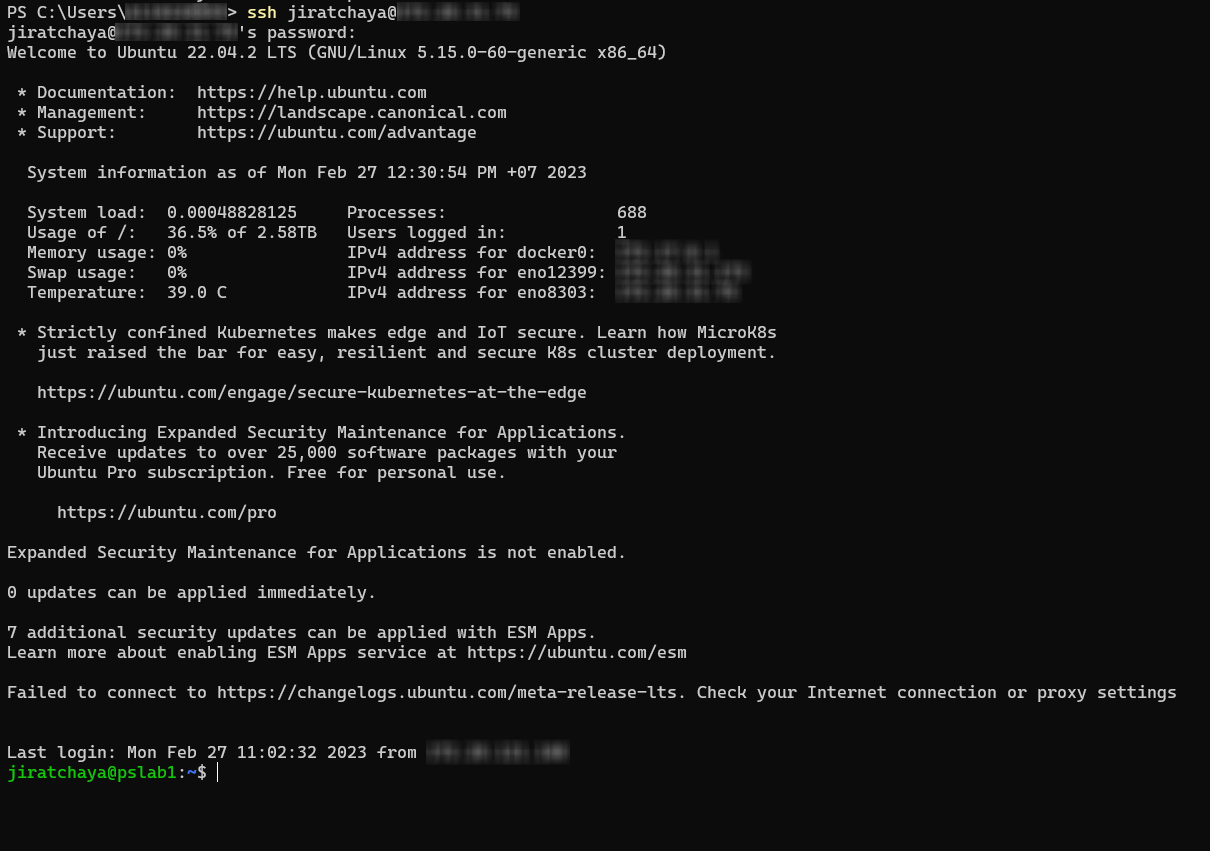
\includegraphics{./assets/03_ssh-welcome-message.png}

}

\caption{An example welcome message of server using Ubuntu, including
general software and hardware status, information of the latest
connection, as well as a prompt for user command.}

\end{figure}

\bookmarksetup{startatroot}

\hypertarget{bash-command-language-for-biologists}{%
\chapter{Bash Command Language for
Biologists}\label{bash-command-language-for-biologists}}

Shell scripting (or shell or UNIX) are heavily used in bioinformatics,
which has been the interface for large bioinformatics programs.
Throughout this workshop, you'll learn how to use the necessary bash
command concepts. This will allow you to focus on the content of
commands in future chapters, rather than be preoccupied with
understanding shell syntax. But before we start to learn bash, it's good
to understand the linux file systems a bit.

\hypertarget{linux-file-systems}{%
\section{Linux File Systems}\label{linux-file-systems}}

Adopted from
\href{https://www.geeksforgeeks.org/linux-file-hierarchy-structure}{linux-file-hierarchy-structure},
In Unix-like operating systems, the Linux File System defines the
directory structure and contents. Even if they're on different physical
or virtual disks, all files and directories are under the root
directory.

\begin{figure}

{\centering \includegraphics{https://media.geeksforgeeks.org/wp-content/uploads/linuxDir.jpg}

}

\caption{Schematic hierarchy of Linux file systems. The figure is
adopted from
https://www.geeksforgeeks.org/linux-file-hierarchy-structure.}

\end{figure}

\begin{description}
\item[Root (\texttt{/})]
It is the root directory of the entire file system hierarchy and the
primary hierarchy root. The root directory is where everything starts.
This directory can only be written by root.
\item[/bin]
Essential commands that need to be available in all users, for example,
\texttt{cat}, \texttt{ls}, \texttt{cp}, \texttt{cd}, \texttt{top},
\texttt{mkdir} and many more.
\item[/dev]
Essential device files such as \texttt{/dev/null}, \texttt{/dev/shm}.
These include terminal devices, usb, or any device attached to the
system.
\item[/etc]
System-wide configuration files for the host, contain files all programs
need. Also included are startup and shutdown shell scripts for starting
and stopping individual programs, such as \texttt{/etc/fstab} for
permanently mounting external disks, \texttt{/etc/netplan} for
configuring the network and IP address, and more.
\item[/home]
The home directories of users, where they keep their saved files and
settings. These directories are used to store all of a user's files and
settings in one place, making it easy for them to access their data and
keep it organized. For example \texttt{/home/ponsit},
\texttt{/home/jiratchaya}, \texttt{/home/prasert}.
\item[/lib]
Contain essential libraries for the binaries in \texttt{/bin/} and
\texttt{/sbin/}.
\item[/media]
Mount points for removable media such as CD-ROMs (deprecated).
\item[/mnt]
Temporary mount directory where sysadmins can mount file systems, such
as \texttt{/mnt/external\_disk\_1}, \texttt{/mnt/removable\_drive\_1},
etc.
\item[/opt]
Optional application software packages. Contains add-on applications
from individual vendors.
\item[/sbin]
Essential system binaries, e.g., \texttt{fsck}, \texttt{init}, route.
\item[/tmp]
Temporary files that aren't preserved between reboots, and may be
severely limited.
\item[/usr]
A secondary hierarchy for read-only user data. The majority of utilities
and apps are in here.
\end{description}

\hypertarget{basic-bash-commands}{%
\section{Basic Bash Commands}\label{basic-bash-commands}}

Bash is a Unix shell that allows you to enter commands, which are then
interpreted and run by the computer. Commands can be used to perform
tasks, such as creating a directory, running a program, or deleting a
file. Bash is a type of interpreter, which takes user input and converts
it into a language that the computer can understand and execute.
Commands are typically composed of keywords, arguments, and flags, which
allow the user to control how the command is interpreted and executed by
the computer.

\begin{itemize}
\tightlist
\item
  \textbf{Navigating your file system}
\end{itemize}

The file system manages files and directories in the operating system,
as shown in the diagram above. It organizes our data into files, which
store information, and directories.

\begin{verbatim}
jiratchaya@pslab1:~$
\end{verbatim}

The dollar sign \texttt{\$} is a prompt, which shows us that the shell
is waiting for input. Your shell may use a different character as a
prompt and may add information before the prompt.

\begin{itemize}
\tightlist
\item
  \textbf{Find out where we are now}
\end{itemize}

\begin{verbatim}
pwd
\end{verbatim}

pwd stand for print working directory. Without explicitly specifying
something else, the computer assumes we want to run commands in our
current working directory. Which can be a user's home directory
(\texttt{\textasciitilde{}}).

\begin{itemize}
\tightlist
\item
  \textbf{Changing directory}
\end{itemize}

\begin{verbatim}
cd your_target_directory
\end{verbatim}

Which stands for change directory. You can change our working directory
by typing \texttt{cd} followed by a directory name. In this case, you
care changing from the current directory to the directory named
\texttt{your\_target\_directory}.

\begin{itemize}
\tightlist
\item
  \textbf{Listing directories}
\end{itemize}

We can see files and subdirectories are in this directory by running ls,
which stands for ``listing'':

\begin{verbatim}
ls
\end{verbatim}

Let's see in the different way. This way is to list all files and
directories including user who belong to, permissions, and file size in
bytes.

\begin{verbatim}
ls -l
\end{verbatim}

To list files and folders, permissions, and size in human-readable
format.

\begin{verbatim}
ls -lh
\end{verbatim}

See all hidden files and directories

\begin{verbatim}
ls -a
# or
ls -la
\end{verbatim}

\hypertarget{resources}{%
\section{Resources}\label{resources}}

\begin{itemize}
\item
  \href{https://hbctraining.github.io/Intro-to-shell-flipped/}{Introduction
  to the command line interface} by Harvard Chan Bioinformatics Core
  (HBC) .
\item
  \href{https://bioinformatics-core-shared-training.github.io/shell-genomics/01-introduction/index.html}{Introducing
  the Shell}, from the course Introduction to the Command Line for
  Genomics in
  \href{https://bioinformatics-core-shared-training.github.io/}{bioinformatics-core-shared-training}
\item
\end{itemize}

\bookmarksetup{startatroot}

\hypertarget{data-retrieval-with-ncbi-sra-tools}{%
\chapter{Data Retrieval with NCBI
sra-tools}\label{data-retrieval-with-ncbi-sra-tools}}

\bookmarksetup{startatroot}

\hypertarget{rna-seq-data-quality-control}{%
\chapter{RNA-Seq Data Quality
Control}\label{rna-seq-data-quality-control}}

\bookmarksetup{startatroot}

\hypertarget{de-novo-assembly-with-trinity}{%
\chapter{De novo Assembly with
Trinity}\label{de-novo-assembly-with-trinity}}

\bookmarksetup{startatroot}

\hypertarget{differential-gene-expression-analysis}{%
\chapter{Differential Gene Expression
Analysis}\label{differential-gene-expression-analysis}}

\bookmarksetup{startatroot}

\hypertarget{references}{%
\chapter*{References}\label{references}}
\addcontentsline{toc}{chapter}{References}

\markboth{References}{References}

\hypertarget{refs}{}
\begin{CSLReferences}{0}{0}
\end{CSLReferences}



\end{document}
